\documentclass[french]{article}
\usepackage{ae, lmodern}
\usepackage[francais]{babel}
\usepackage[utf8]{inputenc}
\usepackage[T1]{fontenc}
\usepackage{todonotes}
\usepackage{fancyhdr}
\usepackage{soul}
\usepackage{ulem}
\usepackage{color}
\usepackage{float}
\usepackage{graphicx}
\usepackage{verbatim}
\usepackage{moreverb}
\usepackage{listings}
\usepackage{url}
\usepackage{array}
\usepackage{longtable}



\title{Simulation sur ordinateur \\ Première session : Rapport \\ Etude du caractère pseudo-aléatoire de $\pi$}
\author{Maazouz Mehdi, Caredda Giuliano \\ BA3 Info}
\date{28 Mai 2018}

\begin{document}
\maketitle
\newpage
\renewcommand{\contentsname}{Sommaire}
\tableofcontents
\newpage

\section{Introduction}
Dans le cadre du cours de \textit{Simulation sur ordinateur} dispensé et corrigé par \textit{Monsieur Alain BYUS}, tous les étudiants sont amenés à réaliser un travail.
\\
\\
Ce dernier consiste à : 
\\

     - Etudier le caractère pseudo-aléatoire des décimales de $\pi$ en utilisant les techniques vues au cours afin de déterminer si ces dernières suivent une loi uniforme.
     \\
     
     -Implémenter un générateur de loi uniforme dans l'intervalle [0,1[ à l'aide des décimales de $\pi$.
     \\
     
     -Comparer ce dernier au générateur par défaut de Python.
\\
\\
Nous avons scindé le projet en 2 parties, la première concerne l'étude du caractère pseudo-aléatoire des décimales
de $\pi$ à l'aide de 3 tests différents.
\\
La deuxième partie concerne non seulement l'explication et l'implémentation de notre générateur aléatoire, mais également sa comparaison avec le générateur par défaut de Python.
\\
\\
\textbf{Remarque :} un fichier contenant le premier million des décimales de $\pi$ nous a été fourni.

\subsection{Logiciels utilisés}
-Le langage de programmation \textbf{Python} dans sa version \textbf{2.7} a été utilisé dans la réalisation de nos différents scripts.
\\

-Le logiciel \textbf{Gnuplot 5.0} nous a servis dans la réalisation des différents histogrammes.
\\

-Le logiciel libre \textbf{TexStudio 5.5.1} nous a permis de rédiger ce rapport.
\\

-Notons enfin l'utilisation de modules de \textbf{Python} tel que \textbf{Math} ou encore \textbf{Sympy}.

\section{Etude de $\pi$ }
\subsection{Approche Naïve}
Pour notre première approche, nous allons tracer un histogramme contenant les occurrences de chacun des digits présents dans notre fichier fourni. Ensuite, nous comparerons ces occurrences observées avec les occurrences théoriques,attendues si nos données suivaient bien une loi uniforme. 
\\
\\
Le nombre d'occurrence théorique de chaque digit peut être calculé assez facilement. En effet, nous avons 10 digits (de 0 à 9), chacun ayant une probabilité valant 1/10 d'apparaître. Comme notre fichier contient 1 000 000 de décimales, la valeur attendue pour chaque digit est de 100 000.
\\
\\
Regardons maintenant notre histogramme et débattons ensuite des premières constatations.

\begin{figure}[h!]
	\hbox to\hsize{\hss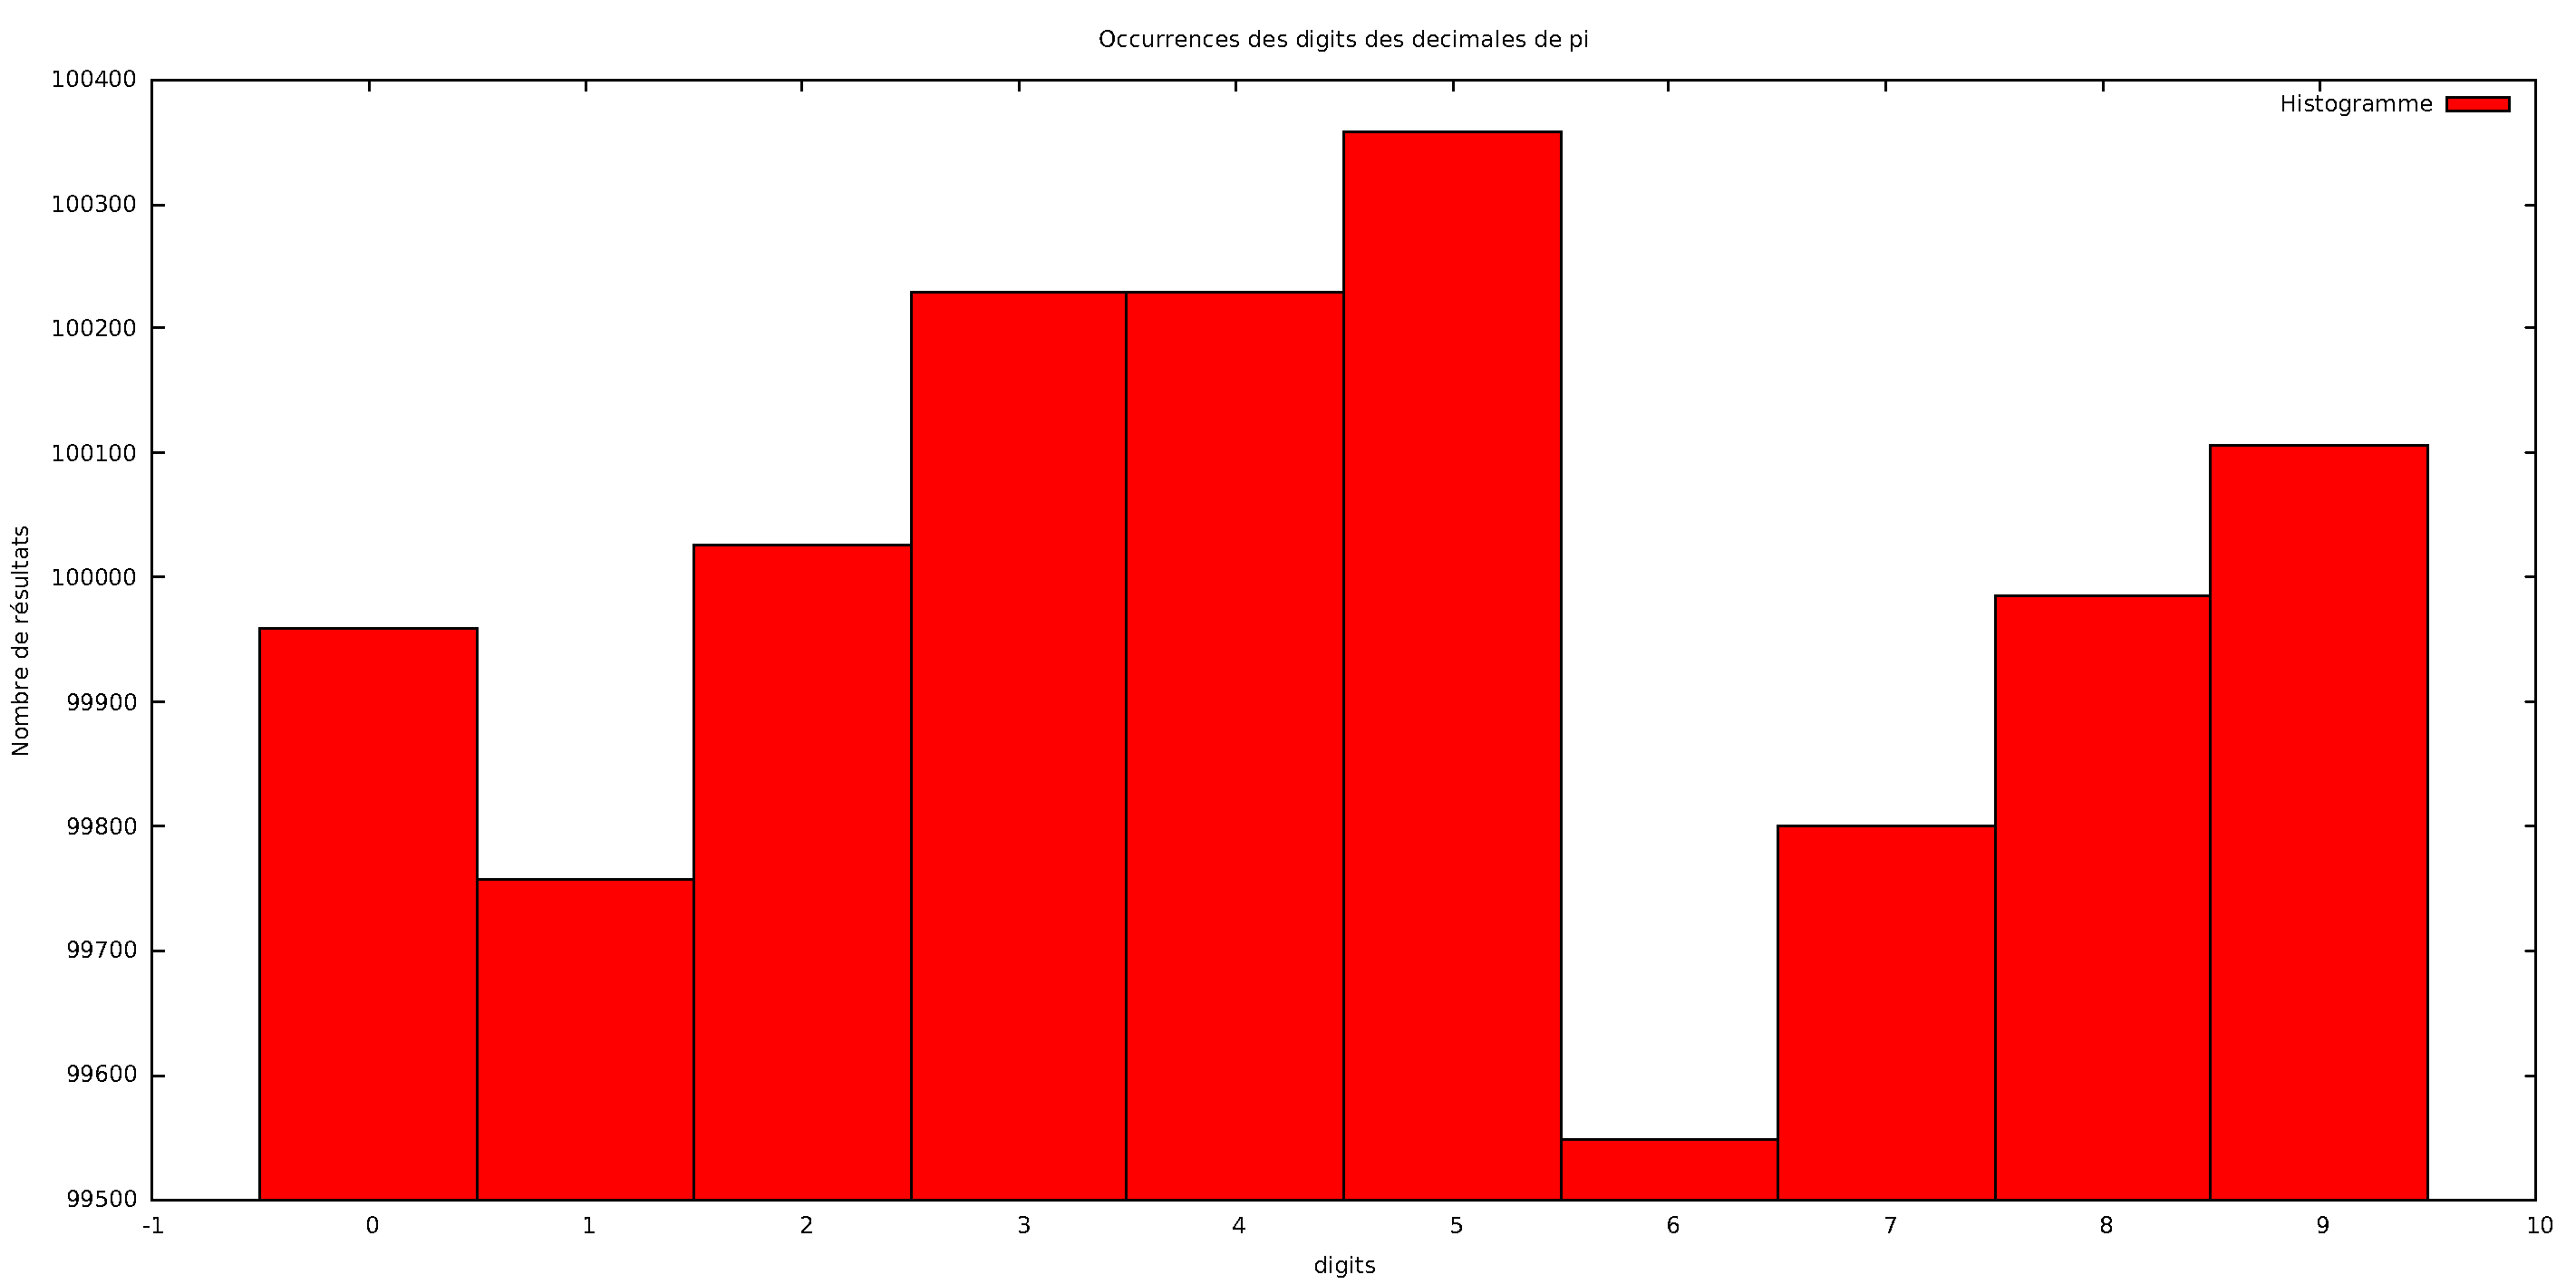
\includegraphics[scale=0.38]{Archives/Images/histo_zoom}\hss}
	\caption{\label{toucan}}
\end{figure}

\newpage
Mettons désormais les données dans un tableau afin de comparer les occurrences obtenues et théoriques.
\begin{longtable}{|c|c|c|c|c|c|c|c|c|c|}
	\hline
	& \multicolumn{3}{c|}{\textbf{Résultats}} \\ 
	\hline 
	\textbf{Digit}  & \textbf{Observé} & \textbf{Attendu} & \textbf{Erreur en \%} \\ 
	\hline 
	$$0$$ & 99 959 & 100 000 & 0.041\\ 
	\hline 
	$$1$$ & 99 758 & 100 000 & 0.24\\ 
	\hline 
	$$2$$ & 100 026 & 100 000 & 0.026 \\ 
	\hline 
	$$3$$ & 100 229 & 100 000 & 0.229\\ 
	\hline 
	$$4$$ & 100 230 & 100 000 & 0.230\\ 
	\hline 
	$$5$$ & 100 359 & 100 000 & 0.359\\ 
	\hline 
	$$6$$ & 99 548 & 100 000 & 0.452\\ 
	\hline 
	$$7$$ & 99 800 & 100 000 & 0.2\\ 
	\hline 
	$$8$$ & 99 985 & 100 000 & 0.015\\ 
	\hline 
	$$9$$ & 100 106 & 100 000 & 0.106\\ 
	\hline
\end{longtable}

On peut constater qu'entre les résultats observés et attendus, il y a à chaque fois une
erreur inférieur à 0,5\%
\\
Ce qui nous encourage à penser que nos données suivent bien une loi uniforme même si cela ne 
constitue pas une preuve.
\\
Passons maintenant à des tests plus complets.
\\
\subsection{Test de $\chi^{2}$ }
Le premier test que nous allons effectuer est le test du \textbf{$\chi^{2}$}. Ce dernier est un test statistique qui va permettre de vérifier si une série de données est susceptible de suivre une loi de probabilité.
\\

\subsubsection{Rappel Théorique}
Afin de vérifier si notre échantillon suit une loi, prenons cette loi comme hypothèse nulle \textit{$H_{0}$}
	\begin{center}
		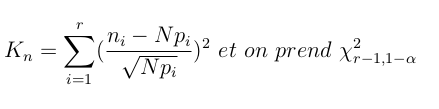
\includegraphics[scale=0.60]{Archives/Images/khi2}
	\end{center}
		
   -\textit{r} correspond au nombre de classes. 
   \\
   -\textit{N$p_{i}$} correspond aux nombres d'occurrences théoriques. 
   \\
   -\textit{$n_{i}$} correspond aux nombres d'occurrences observées.
   \\
   -Le paramètre \textit{$\alpha$} représente l'erreur de première espèce, autrement dit, la probabilité de rejeter l'hypothèse nulle \textit{$H_{0}$} alors que cette dernière est vraie.
   \\
   -$\chi^{2}_{\textit{r}-1,\alpha-1}$ le degré de liberté.
\\
\\
Si \textit{$K_{n}$} <$\chi^{2}$, alors on accepte notre hypothèse nulle.
\\
Si \textit{$K_{n}$} > $\chi^{2}$, on la rejette.
\\
\subsubsection{Mise en pratique}
Partons désormais de notre hypothèse nulle :
\\
\\
       $H_{0}$ = {nos décimales suivent une loi uniforme}.
\\
\\
De plus : 
\\
\\
     -\textit{r} sera fixé à 10, car nous considérerons une classe par digit.
     \\
     -\textit{N$p_{i}$} sera fixé à 100 000.
     \\ 
     -Quant à \textit{$n_{i}$}, ses différentes valeurs seront issues du nombre d'occurrence observés dans l'histogramme présenté précédemment.
     \\
     -$\chi^{2}_{9,\alpha-1}$ où 9 est le degré de liberté calculé en faisant \textit{r}-1 (nombre de classes -1).
\\

Voici les différents résultats obtenus en fonction de différentes valeurs pour $\alpha$.
\\
\begin{longtable}{|c|c|c|c|c|c|c|c|c|c|}
	\hline
	& \multicolumn{3}{c|}{\textbf{Résultats}} \\ 
	\hline 
	\textbf{$\alpha$}  & $K_{n}$ & $\chi^{2}_{9,\alpha-1}$ & \textbf{Resultat} \\ 
	\hline 
	$$0.001$$ & 5.50908 & 27.877 & Reussite\\ 
	\hline 
	$$0.025$$ & 5.50908 & 19.023 & Reussite\\ 
	\hline 
	$$0.1$$ & 5.50908 & 14.684 & Reussite \\ 
	\hline 
\end{longtable}

Nous pouvons constater que tous les tests ont réussi, nous sommes donc confortés dans notre supposition qui était que les décimales de $\pi$ suivent une loi uniforme.
\\

\subsection{Test du Poker}
Une fois le test du $\chi^{2}$ effectué, passons maintenant à un autre test qui va s'appuyer sur ce dernier, le test du Poker. 
\\
\\
Premièrement, nous allons diviser notre million de décimales en 200 000 blocs contenant chacun 5 décimales. Nous dirons que chaque bloc contient une séquence.
\\
\\
Une fois les blocs obtenus, nous allons les classer en fonction du nombre de digit différents par bloc. Ce nombre est appelé \textit{r} et est compris entre 1 et 5.
\\
En effet, une séquence peut ne contenir qu'un digit différent (par exemple : 11111) mais également 5 digits différents (12345).
\\
\\
Ensuite, nous passerons au calcul du $\chi^{2}$ afin de comparer les occurrences obtenues pour chaque \textit{r} avec les occurrences théoriques.
\\
\\
Afin d'obtenir les occurrences théorique, nous allons devoir calculer $P_{r}$, autrement dit, la probabilité d'avoir \textit{r}.
	\begin{center}
		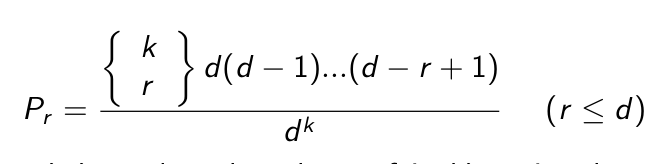
\includegraphics[scale=0.40]{Archives/Images/probaR}
	\end{center}

Avec :
\\
\\
	-\textit{K} la longueur de la séquence.
	\\
	-\textbf{d} le nombre de digits possibles.
	 \\
	-\textbf{r} le nombre de digits différents.
\\
\\
\textbf{Remarque} : nous pouvons constater que $P_{r}$ se base sur le nombre de \textit{Stirling}.
\\
Ce dernier se définit comme étant le \textit{nombre de manières possibles de constituer r paquets avec k nombres}.

	\begin{center}
		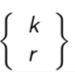
\includegraphics[scale=0.40]{Archives/Images/stirling}
	\end{center}

Les valeurs suivantes ont pu facilement être déterminées par les explications ci-dessus :
\\
\\
	-\textit{K} = 5.
	\\
	-\textbf{d} = 10.
\\
\\
Une fois $P_{r}$ calculé pour chaque \textit{r}, multiplions ces dernières par le nombre de paquet total (200 000) pour avoir les occurrences théoriques.

\begin{longtable}{|c|c|c|c|c|c|c|c|c|c|}
	\hline
	& \multicolumn{3}{c|}{\textbf{Résultats}} \\ 
	\hline 
	\textit{r}  & Occurrence observée & Occurrence théorique \\
	\hline 
	1 & 13  & 20\\
	2 & 2644 & 2700 \\
	3 & 36172 & 36000\\
	4 & 100670 & 100800\\
	5 & 60501  & 60480\\ 
	\hline 
\end{longtable}

\newpage
	\begin{figure}[h!]
		\hbox to\hsize{\hss	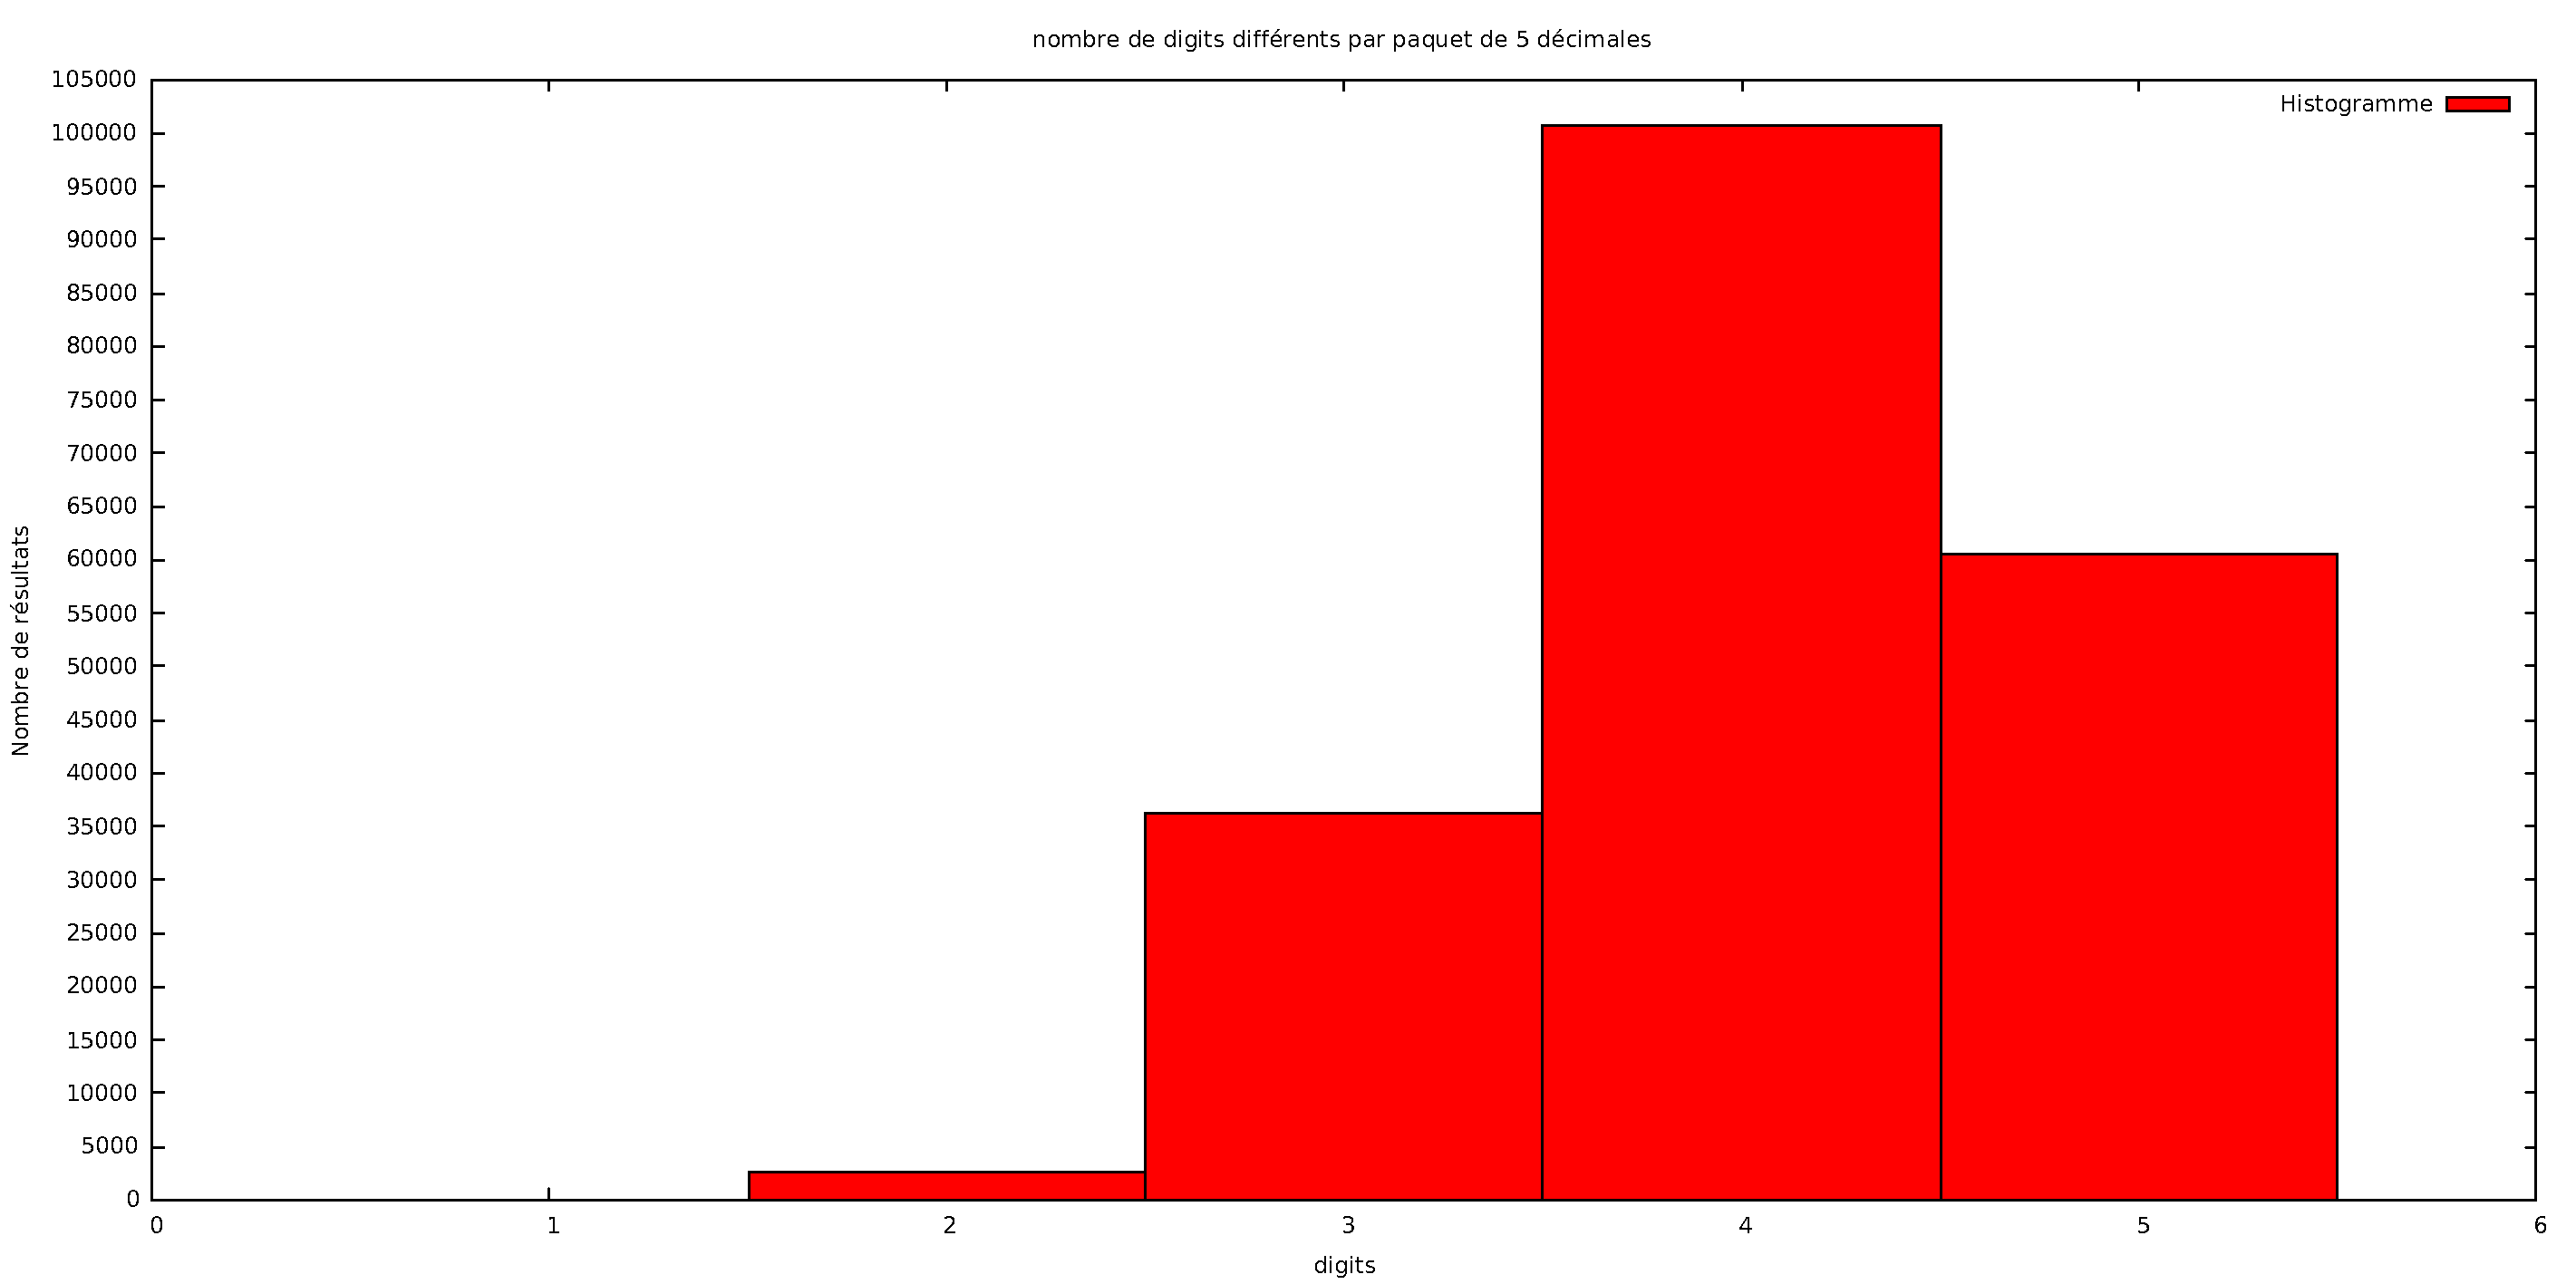
\includegraphics[scale=0.40]{Archives/Images/histo_poker}\hss}
		\caption{\label{toucan}}
	\end{figure}

Après avoir adapté les différents paramètres, passons désormais au test de $\chi^{2}$
\begin{longtable}{|c|c|c|c|c|c|c|c|c|c|}
	\hline
	& \multicolumn{3}{c|}{\textbf{Résultats}} \\ 
	\hline 
	\textbf{$\alpha$}  & $K_{n}$ & $\chi^{2}_{4,\alpha-1}$ & \textbf{Resultat} \\ 
	\hline 
	$$0.001$$ & 4.608 & 18.467 & Reussite\\ 
	\hline 
	$$0.025$$ & 4.608 & 11.143 & Reussite\\ 
	\hline 
	$$0.1$$ & 4.608 & 7.779 & Reussite \\ 
	\hline 
\end{longtable}

Encore une fois, tous les tests ont réussis.
\\
\subsection{Test du collectionneur de coupons}
Le dernier test que nous allons employer repose sur le principe suivant. 
\\
\\
Tout d'abord, nous allons parcourir les décimales de $\pi$ avec pour objectif de construire des séquences.
Une séquence étant construite dès que l'on a parcouru une fois tous les digits possible (de 0 à 9 compris).
Il suffit ensuite de recommencer la procédure avec les décimales suivantes.
\\
On peut facilement comprendre que nous obtiendrons des séquences avec des tailles différentes.
\\
Une fois fait, nous comparerons les occurrences observées pour chaque taille de séquence avec celles théorique grâce au test de \textbf{$\chi^{2}$}.
\\
\\
Afin d'obtenir les occurrences théoriques, nous devons tout d'abord calculé la probabilité $S_{r}$, autrement dit, la probabilité d'avoir une séquence de taille \textit{r} ayant tous nos digits est donnée par la formule suivante :

	\begin{center}
		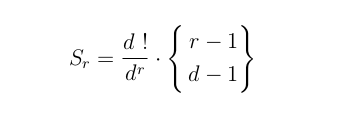
\includegraphics[scale=0.40]{Archives/Images/coupons}
	\end{center}

Avec :
\\
	-\textit{d} représente le nombre de digits possibles, ici, il sera égal à 10.
	\\
	-\textit{r} la taille de la séquence.
\\
\\
Afin d'obtenir la valeur théorique pour chaque taille de séquence \textit{$ r_{i} $}, il suffit de multiplier la probabilité $S_{r_{i}}$  par le nombre total de séquences obtenues.
\\


Nos longueurs de séquences formeront nos classes pour le test de $\chi^{2}$. Nous avons 100 classes, cependant, les séquences ayant une taille allant de 1 à 9 ont une valeur théorique et observée de 0. Elles sont donc inutiles à prendre en considération pour le test de $\chi^{2}$.
\\
Le degré de liberté sera donc égal à 91-1($\chi^{2}_{90,\alpha-1}$).
\newpage
\begin{figure}[h!]
	\centering
	\begin{tabular}{|r|r|r|}
		\hline
		Tailles de séquences & Valeur théorique & Valeur observée\\
		\hline
		10 & 12.39706944 & 12\\
		11 & 55.78681248 & 62\\
		12 & 143.186152032 & 154\\
		13 & 276.144721776 & 265\\
		14 & 445.677125782 & 496\\
		15 & 636.605631934 & 645\\
		16 & 832.196551932 & 869\\
		17 & 1017.53193425 & 1008\\
		18 & 1181.29471772 & 1150\\
		19 & 1316.26375399 & 1341\\
		20 & 1418.98670105 & 1354\\
		21 & 1489.0470501 & 1482\\
		22 & 1528.21745078 & 1576\\
		23 & 1539.67053158 & 1515\\
		24 & 1527.32748565 & 1543\\
		25 & 1495.36642995 & 1456\\
		26 & 1447.88033297 & 1470\\
		27 & 1388.65981367 & 1345\\
		28 & 1321.07229861 & 1317\\
		29 & 1248.01086229 & 1224\\
		30 & 1171.89036844 & 1145\\
		31 & 1094.67343335 & 1105\\
		32 & 1017.91330149 & 1018\\
		33 & 942.804564011 & 968\\
		34 & 870.235668768 & 883\\
		35 & 800.839427633 & 817\\
		36 & 735.039345563 & 772\\
		37 & 673.090709825 & 680\\
		38 & 615.116112395 & 640\\
		39 & 561.135537135 & 522\\
		40 & 511.091408294 & 506\\
		41 & 464.869130432 & 456\\
		42 & 422.313697469 & 406\\
		43 & 383.242942754 & 379\\
		44 & 347.457965104 & 351\\
		45 & 314.751212876 & 324\\
		46 & 284.912648965 & 280\\
		47 & 257.734360295 & 266\\
		48 & 233.013919451 & 219\\
		49 & 210.556755384 & 212\\
		50 & 190.177745431 & 185\\
		\hline
	\end{tabular}
	\caption{Tableau de Test du CDC : Les décimales de Pi 1}
\end{figure}

\newpage
\begin{figure}[h!]
	\centering
	\begin{tabular}{|r|r|r|}
		\hline
		Tailles de séquences & Valeur théorique & Valeur observée\\
		\hline
		51 & 171.702202299 & 197\\
		52 & 154.966396843 & 142\\
		53 & 139.817729962 & 148\\
		54 & 126.114644036 & 115\\
		55 & 113.726345551 & 113\\
		56 & 102.532395165 & 87\\
		57 & 92.4222090177 & 95\\
		58 & 83.294505053 & 77\\
		59 & 75.0567200775 & 80\\
		60 & 67.624416886 & 69\\
		61 & 60.9206957291 & 66\\
		62 & 54.8756204189 & 62\\
		63 & 49.4256662748 & 59\\
		64 & 44.5131947077 & 44\\
		65 & 40.0859574053 & 39\\
		66 & 36.0966316837 & 34\\
		67 & 32.5023875297 & 32\\
		68 & 29.2644860878 & 22\\
		69 & 26.3479087976 & 22\\
		70 & 23.7210160015 & 27\\
		71 & 21.3552335886 & 25\\
		72 & 19.2247660837 & 27\\
		73 & 17.3063345114 & 17\\
		74 & 15.5789373362 & 8\\
		75 & 14.0236327962 & 12\\
		76 & 12.6233409926 & 12\\
		77 & 11.3626641589 & 5\\
		78 & 10.2277236148 & 13\\
		79 & 9.20601199223 & 9\\
		80 & 8.28625941323 & 12\\
		81 & 7.45831238842 & 8\\
		82 & 6.71302429704 & 7\\
		83 & 6.04215639528 & 8\\
		84 & 5.43828838508 & 4\\
		\hline
	\end{tabular}
	\caption{Tableau de Test du CDC : Les décimales de Pi 3}
\end{figure}

\begin{figure}[h!]
	\centering
	\begin{tabular}{|r|r|r|}
		\hline
		Tailles de séquences & Valeur théorique & Valeur observée\\
		\hline
		85 & 4.89473765491932 & 4\\
		86 & 4.40548637952699 & 5\\
		87 & 3.96511573604793 & 6\\
		88 & 3.56874655969782 & 3\\
		89 & 3.21198582270483 & 1\\
		90 & 2.89087837643692 & 0\\
		91 & 2.60186344817007 & 1\\
		92 & 2.34173543125690 & 4\\
		93 & 2.10760855073593 & 4\\
		94 & 1.89688502594326 & 0\\
		95 & 1.70722638771169 & 1\\
		96 & 1.53652764052733 & 1\\
		97 & 1.38289398981167 & 4\\
		98 & 1.244619881547491 & 0\\
		99 & 1.12017012599947 & 2\\
		\hline
	\end{tabular}
	\caption{Tableau de Test du CDC : Les décimales de Pi 3}
\end{figure}
\newpage
Nous pouvons constater que le tableau affiche les résultats à partir des séquences de longueur 10. En effet, il est inutile de prendre en considération les séquences de longueur inférieure à 10 car il est impossible de trouver une séquence contenant les 10 digits différents (0 à 9) si la séquence a une longueur inférieure à 10.
\\
\\
Voici les résultats obtenues une fois le test de $\chi^{2}$ effectué :
\begin{longtable}{|c|c|c|c|c|c|c|c|c|c|}
	\hline
	& \multicolumn{3}{c|}{\textbf{Résultats}} \\ 
	\hline 
	\textbf{$\alpha$}  & $K_{n}$ & $\chi^{2}_{9,\alpha-1}$ & \textbf{Resultat} \\ 
	\hline 
	$$0.001$$ & 78.792 & 137.21 & Reussite\\ 
	\hline 
	$$0.025$$ & 78.792 & 118.14 & Reussite\\ 
	\hline 
	$$0.1$$ & 78.792 & 107.57 & Reussite \\ 
	\hline 
\end{longtable}

\subsection{Conclusion}
Tous les tests qui ont été effectués et qui avaient pour but de déterminer si les décimales de $\pi$ suivaient bien une loi uniforme ont été concluants. Et ce, malgré les différentes marges d'erreurs que nous avions définis avec le paramètre $\alpha$.
\\
\\
Nous pouvons donc affirmer, que d'après ces tests, les décimales de $\pi$ suivent une loi uniforme.
\newpage
\section{Générateur de nombre pseudo-aléatoire}
\subsection{Enonce}
La deuxième partie de notre projet consiste à implémenter un générateur de nombre pseudo-aléatoire et ensuite, de le comparer avec le générateur par défaut de Python (Mersenne Twister). Plus concrètement, nous devons implémenter un générateur qui devra, comme son nom l'indique, générer des nombres compris entre 0 et 1
de manière uniforme.

\subsection{Implémentation}
Nous savons que l'ordinateur est une machine déterministe. Cependant, nous pouvons faire ressortir une composante aléatoire en utilisant le temps écoulé, en millisecondes, depuis le $1^{er}$ Janvier 1970.
\\
Etant donné que les premières décimales de  $\pi$ nous sont fournies, nous allons pouvoir nous en servir pour l'implémentation de notre générateur.
\end{document}
